
%(BEGIN_QUESTION)
% Copyright 2007, Tony R. Kuphaldt, released under the Creative Commons Attribution License (v 1.0)
% This means you may do almost anything with this work of mine, so long as you give me proper credit

All devices fail -- it is not a question of ``if,'' but ``when.''  Given this fact, it is logical to provide dangerous processes with {\it redundant} control components, so that system safety is never dependent on any single component.

For example, suppose we wished to equip a furnace with a high-temperature safety shutdown system, to shut off fuel to the burner if ever the furnace temperature reached some critical value.  Here, two high-temperature switches control two fuel shutoff valves.  Both switches have the same trip point, and both solenoid valves work identically:

$$\includegraphics[width=15.5cm]{i02487x01.eps}$$

\filbreak

Here is another high-temperature shutdown system using redundant sensors and redundant safety valves.  However, this system will not function the same as the previous system:

$$\includegraphics[width=15.5cm]{i02487x02.eps}$$

Determine which of these two redundant shutdown systems provides the greatest level of {\it dependability} (i.e. preventing over-temperature of the furnace), and which of them provides the greatest level of {\it security} (i.e. the ability to continue running the furnace when there is no overtemperature condition).

\underbar{file i02487}
%(END_QUESTION)





%(BEGIN_ANSWER)

The first (series valves) system provides 1oo2 dependability and 2oo2 security.  The second (parallel valves) system provides 2oo2 dependability and 1oo2 security.

%(END_ANSWER)





%(BEGIN_NOTES)


%INDEX% Safety, redundancy: availability versus safety

%(END_NOTES)


